
\begin{figure*}[t]
    \centering
    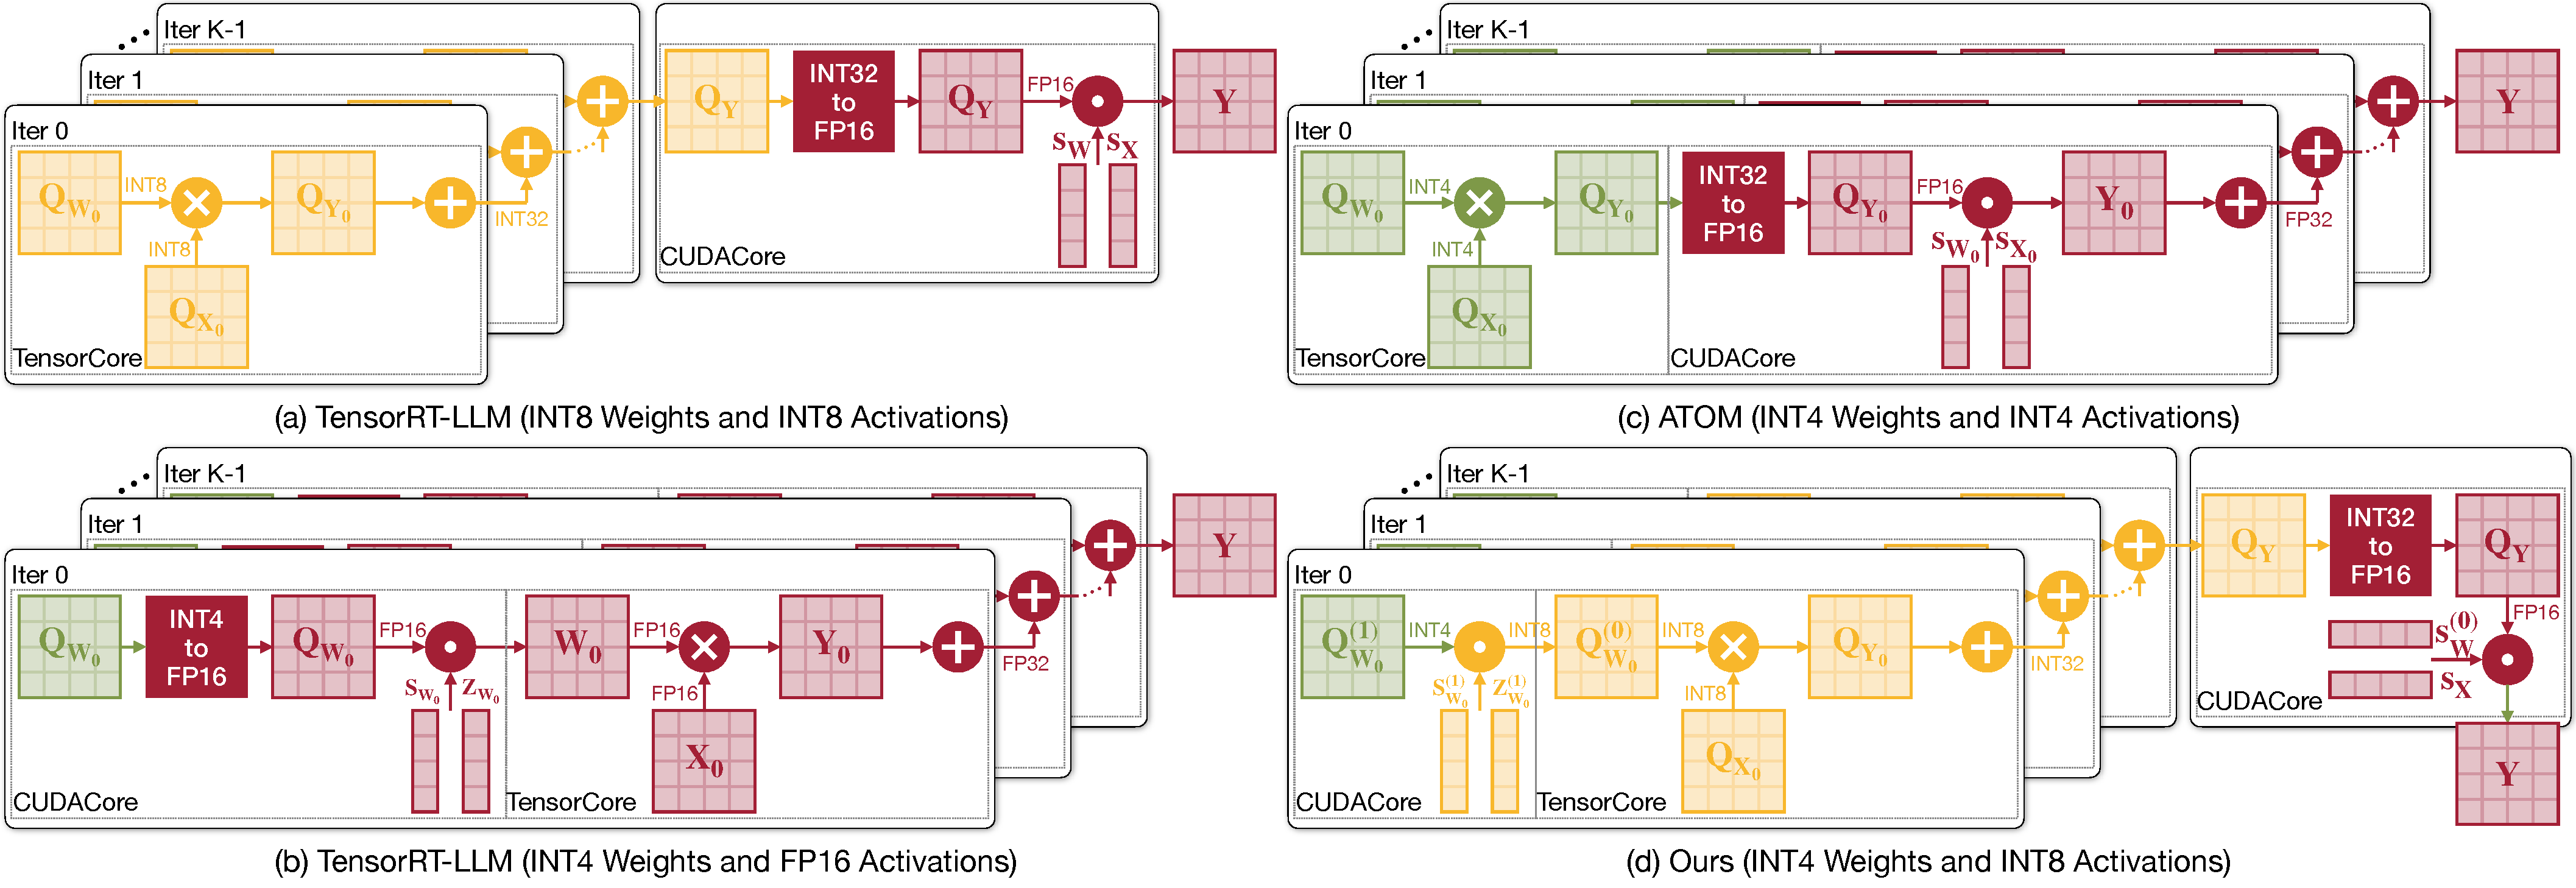
\includegraphics[width=\linewidth]{figure/3-motivation/gemm-flow-compare-2x2.pdf}
    \caption{\textbf{Quantized GEMM on GPUs:} \textbf{\texttt{W8A8}} is fast because its main loop only contains \textit{tensor core} operations and all dequantization operations are present in the epilogue. Atom-\textbf{\texttt{W4A4}} and TensorRT-LLM-\textbf{\texttt{W4A16}} suffer from significant partial sum or weight dequantization overhead in the main loop. Thanks to the two-level progressive quantiation algorithm, \system-\textbf{\texttt{W4A8}} reduces main loop dequantization overhead by introducing register-level parallelism.}
    \label{fig:motivation:gemm}
    \vspace{-8pt}
\end{figure*}
